\section{\textbf{EnDASH System}}\label{section:sys_overview}
%\basabdatta{\textbf{The first two paragraphs are repetitions. Can be clubbed into one.}}\\ \niloy{Completely remove this - start with OVerview and just write a line that the module is in cloud. }
 %Its objective is to improve the energy efficiency of \ac{ABR} video streaming in smartphones connected to cellular networks, while not compromising on the \ac{QoE} of individual users, especially under mobility conditions. Existing \ac{ABR} algorithms \cite{Yin2015,mao2017neural,Spiteri2016,Akhtar2018,Sengupta2018} mostly focus on \ac{QoE} improvement only, while not concerning about energy savings. These algorithms use a number of inputs, such as playback buffer occupancy, throughput estimate of future chunks, etc. to obtain the current estimate of the supported throughput to decide on the bitrate of the next chunk, such that the user's \ac{QoE} improves. Some SoA algorithms, such as Pensieve \cite{mao2017neural},  involves  computations like training neural networks for optimal bitrate selections. \\
%\indent Implementation of these algorithms in the client player itself may be limited by the resource. To alleviate this problem, the algorithms are run in external stateless \ac{ABR} servers which provides the bitrates of the next chunks. According to \cite{mao2017neural}, the server being available locally, the latency involved in the communication between the server and the controller is negligible.  Besides, as the server is stateless, it can serve multiple clients with different service requests, while not incurring any additional overhead. 
%\subsection{Overview of the EnDASH system} \indent 
The proposed EnDASH system is an energy efficient client video player, working as a wrapper over \ac{DASH}. It predicts the cellular network throughput over a finite future time window to take decisions on the opportune fetching of  video chunks.  EnDASH operates in a time-slotted fashion. So, the entire timeline is divided into discrete time-slots of length \mq{T}.
%executes the following functions to achieve energy efficient video download: (i) predicts the cellular network link throughput from radio related parameters, (i) determines the length of the playback-buffer using the predicted throughput s.t. energy consumption is minimized, and (iii) decides on the optimal bitrates at which the next video chunks will be downloaded.\\ 
%Correspondingly, EnDASH has three prediction modules. %in the EnDASH architecture are- (i)a network throughput prediction entity, (ii)a buffer decision engine, and (iii) the bitrate selection engine. EnDASH employs an \ac{RF} algorithm for throughput prediction. Subsequently, it uses two asynchronously running \ac{RL} modules, one for determining the buffer length from the average predicted throughput, and one for determining the bitrate of the next chunk.\\ \indent 
 %It is shown in Fig. \ref{fig:EnDASH_timing_diag} that in the 
EnDASH executes the following functions to achieve energy efficient video download: (i) At the beginning of each time slot it uses historical data on radio parameters to predict the cellular network link throughput of the current time slot using a Random Forest Learning (RFL) engine. (ii) It then uses the predicted throughput to predict the optimal playback-buffer length for the current slot that minimizes energy consumption. For this, EnDASH employs the state-of-the-art \ac{A3C} deep \ac{RL} algorithm.  (iii) Before downloading each video chunk within a time slot, EnDASH runs another A3C based deep \ac{RL} engine to predict the optimal download chunk  bitrate. 
% uses the predicted optimal buffer length to decide the optimal bitrates at which the next video chunks will be downloaded. , EnDASH runs - (a)  (b) to select an {\bf optimal buffer length}, in terms of the number of seconds of video to be played, using the predicted throughput. The reward function of the buffer length decision engine is a linear weighted function of the savings in energy and QoE score. 
% Once the buffer length is decided, the number of chunks that will be downloaded in the corresponding slot is determined. EnDASH then initiates a second deep RL-based {\bf optimal bitrate decision engine}, which runs multiple times within a timeslot specifically before downloading each video chunk. %So, the EnDASH system has two deep-RL driven neural networks running asynchronously. 
 %In the first time slot, EnDASH behaves in the same way as an \ac{ABR} algorithm which selects optimal bitrates for downloading the next video chunk using a neural network, like Pensieve \cite{mao2017neural}. 
 EnDASH is, thus, a cascaded system of three engines: (i) throughput prediction, (ii) buffer length decision,  and (iii) bitrate selection as shown in Fig. \ref{fig:EnDASH system}. We next describe these modules.% in detail.
%  \begin{figure}[t]
% 	\centering
% 	\includegraphics[width = 0.5\textwidth,trim = {1cm 6cm 3cm 2cm}]{figures/ENDASH_timing_diag.pdf}
% 	\caption{Timing Diagram of EnDASH system; time-axis is divided intro slots of equal length \mq{T}. Throughput prediction and buffer length decisions are taken at the end of each time slot as marked by arrows.}
% 	\label{fig:EnDASH_timing_diag}
% \end{figure}
 \begin{figure}[t]
	\centering
	\includegraphics[width = 0.9\textwidth,trim = {1cm 1cm 1cm 1cm}]{figures/EnDASH_system.pdf}
	\caption{Composite Representation of the EnDASH model; a cascaded model where the predicted throughput acts as an input network state to the Actor Critic \ac{RL} based decision engine}
	\label{fig:EnDASH system}
\end{figure}
 \subsection{The Throughput Prediction Engine}\label{section:thpre}
% \niloy{Very poorly written, needs to discuss before correcting}
EnDASH employs a \ac{RFL} algorithm for cellular network throughput prediction ~\cite{Raca2019}. At the beginning of time slot \mq{t}, it uses the historical information of different radio related parameters in the previous \mq{x} seconds to predict the average throughput~\footnote{Since video rate adaptation algorithms mostly use average throughput, hence for EnDASH, we have predicted the average throughput only \cite{Raca2019}.} that may be experienced by the user during the time slot (of length `T'). We represent this as $\prefu{x}{T}$. 
%Effects of varying \mq{x} and \mq{T} on prediction accuracy, \ac{QoE} score, energy consumption, etc., has been investigated extensively and reported in \S\ref{section:evaluation}.  The data used for the prediction involves radio metrics and measured throughput, captured in our w
The input features of the throughput prediction engine are: (i) \ti{RSSI}, (b) \ti{technologies used} - LTE (4G), HSPA+ (3.75G), UMTS (3G), EDGE (2G), (c) \ti{number of vertical and horizontal \ti{handovers}}, (d) \ti{speed},  (e) \ti{number and technology of neighbouring \acp{BS}}, (f) \ti{download link throughput} - the download rate is measured at the \ac{UE} in bytes per second. Readings on these features  are obtained from the NetMonitor Lite app with a granularity of one second.\\
%(The number of neighbouring \acp{BS} is particularly important for \ac{4G} which uses frequency reuse.)
 %\indent EnDASH is targeted towards improving battery power consumption across all cellular network technologies. So, for throughput prediction in EnDASH we have used only those parameters which are quantified for all technologies. Such parameters, which influence the throughput and has been used in our work, are enlisted below:
 %\begin{enumerate}
  %   \item \textbf{RSSI}: \ac{RSSI} quantifies the strength of the received signal. \item \textbf{Associated Technology}: When a \acp{UE} falls back to legacy 3G and 2G networks, it experiences a throughput  much less 4G.  \item \textbf{Handover Events}: We consider both horizontal handover events between \acp{BS} of the same technology and vertical handovers between \acp{BS} of different technologies. \item \textbf{Speed}: The higher is the speed, the higher is the effect of Doppler  spread \cite{Stuber2001} \item \textbf{Number of neighbouring \acp{BS}}: Neighbouring \acp{BS} may be \ac{4G} \acp{eNB} or 3G NodeBs or 2G \acp{BS}. The number of neighbouring \acp{BS} is particularly important for \ac{4G} which uses frequency reuse one. \item \textbf{Download link throughput}: This is the download rate measured at the \ac{UE}.\end{enumerate}
\indent  Each feature can be represented as a distribution, 
 %\paragraph{Implementation} Classical machine learning algorithms can achieve a high degree of accuracy  when fed with high level features obtained of the raw input data. So, 
 However, instead of feeding the entire time-series data for each metric, we adopt the summarization technique of \cite{Raca2019}. So, we feed only a few key values that best summarize the data and its corresponding distribution. %\cite{Raca2019} suggests that the empirical distribution of any unknown data is best summarized by its inter-quartile range, 90$^{th}$ percentile point, and the mean. Thus, for any metric, 
 For each of the features we obtain the $\mathrm{25^{th}}$, $\mathrm{75^{th}}$, and $\mathrm{90^{th}}$ percentile points, median and mean from its historical data and feed it to the \ac{RFL} algorithm. We train and test this module using 39662 seconds of collected data on received throughput across five Indian cities.
 % in India (Kharagpur, Kolkata, Guwahati, Bengaluru, Malda) for throughput prediction.
 %\niloy{Discuss with Abhijit. }
%  \indent As our objective is to provide seamless service under mobility conditions, we primarily train the RF algorithm using the datasets on mobility that we have collected. These datasets correspond to those of file download. We have collected nearly 100 traces of data using two phones, each operating under different service providers over a period of three months. We have generated the traces while downloading both 6Mb and 100 Mb file sizes. The error in prediction of the RF algorithm is quantified as follow:
%  \begin{equation}
%      \hat{e} = \sqrt{\frac{1}{N}\sum_{i=1}^N\left(\mathrm{max}(10,R_i)-\mathrm{max}(10,\hat{R_i})\right)^2}
%  \end{equation}
%   \begin{figure*}[t]%
% \centering
% \subfigure[Shows the feature importance of the input parameters; signal strength, associated technology, and handovers between technology are the three features having the highest contribution in deciding throughput]{%
% \label{fig:feature_imp}%
% 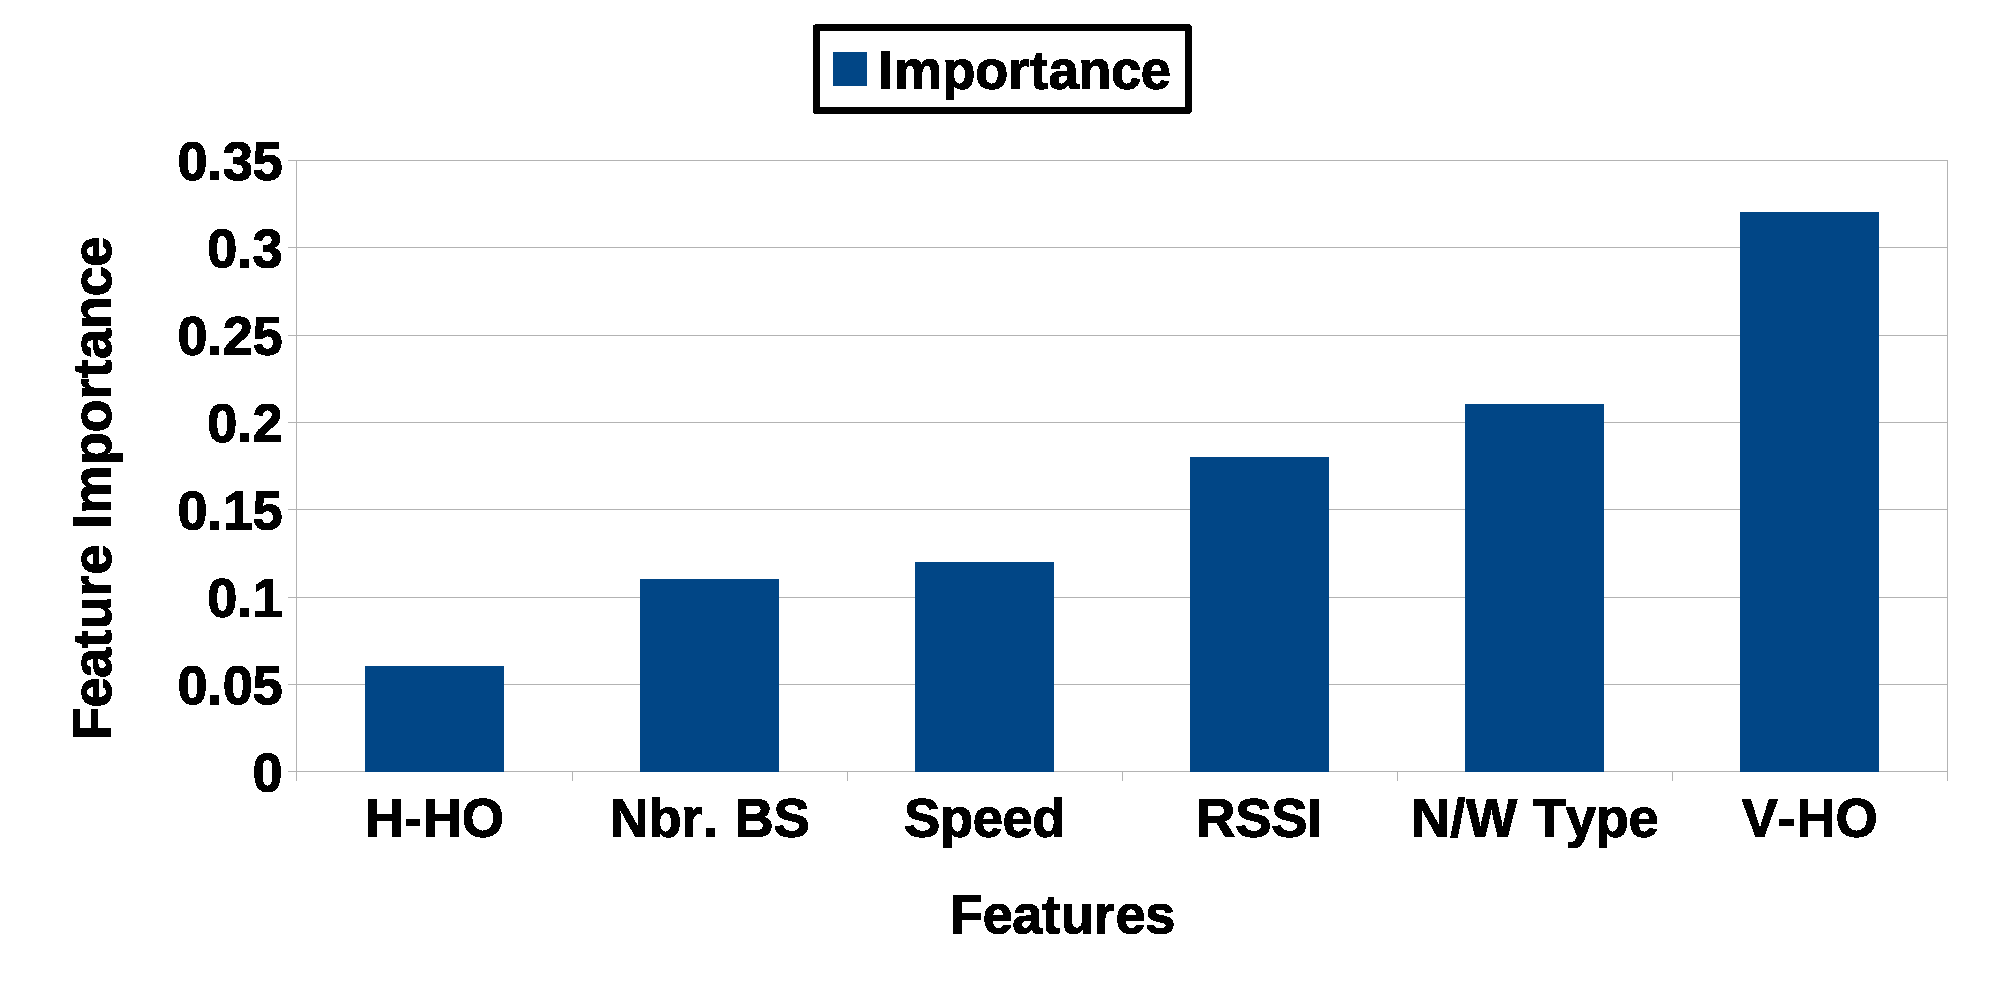
\includegraphics[width=0.3\textwidth]{figures/Feature_importance.eps}}%
% %\hspace{0.1cm}
% \subfigure[The Predicted vs the Actual throughput using the RF algorithm when associated technology is considered.]{%
% \label{fig:thpt_pred_trace}%
% 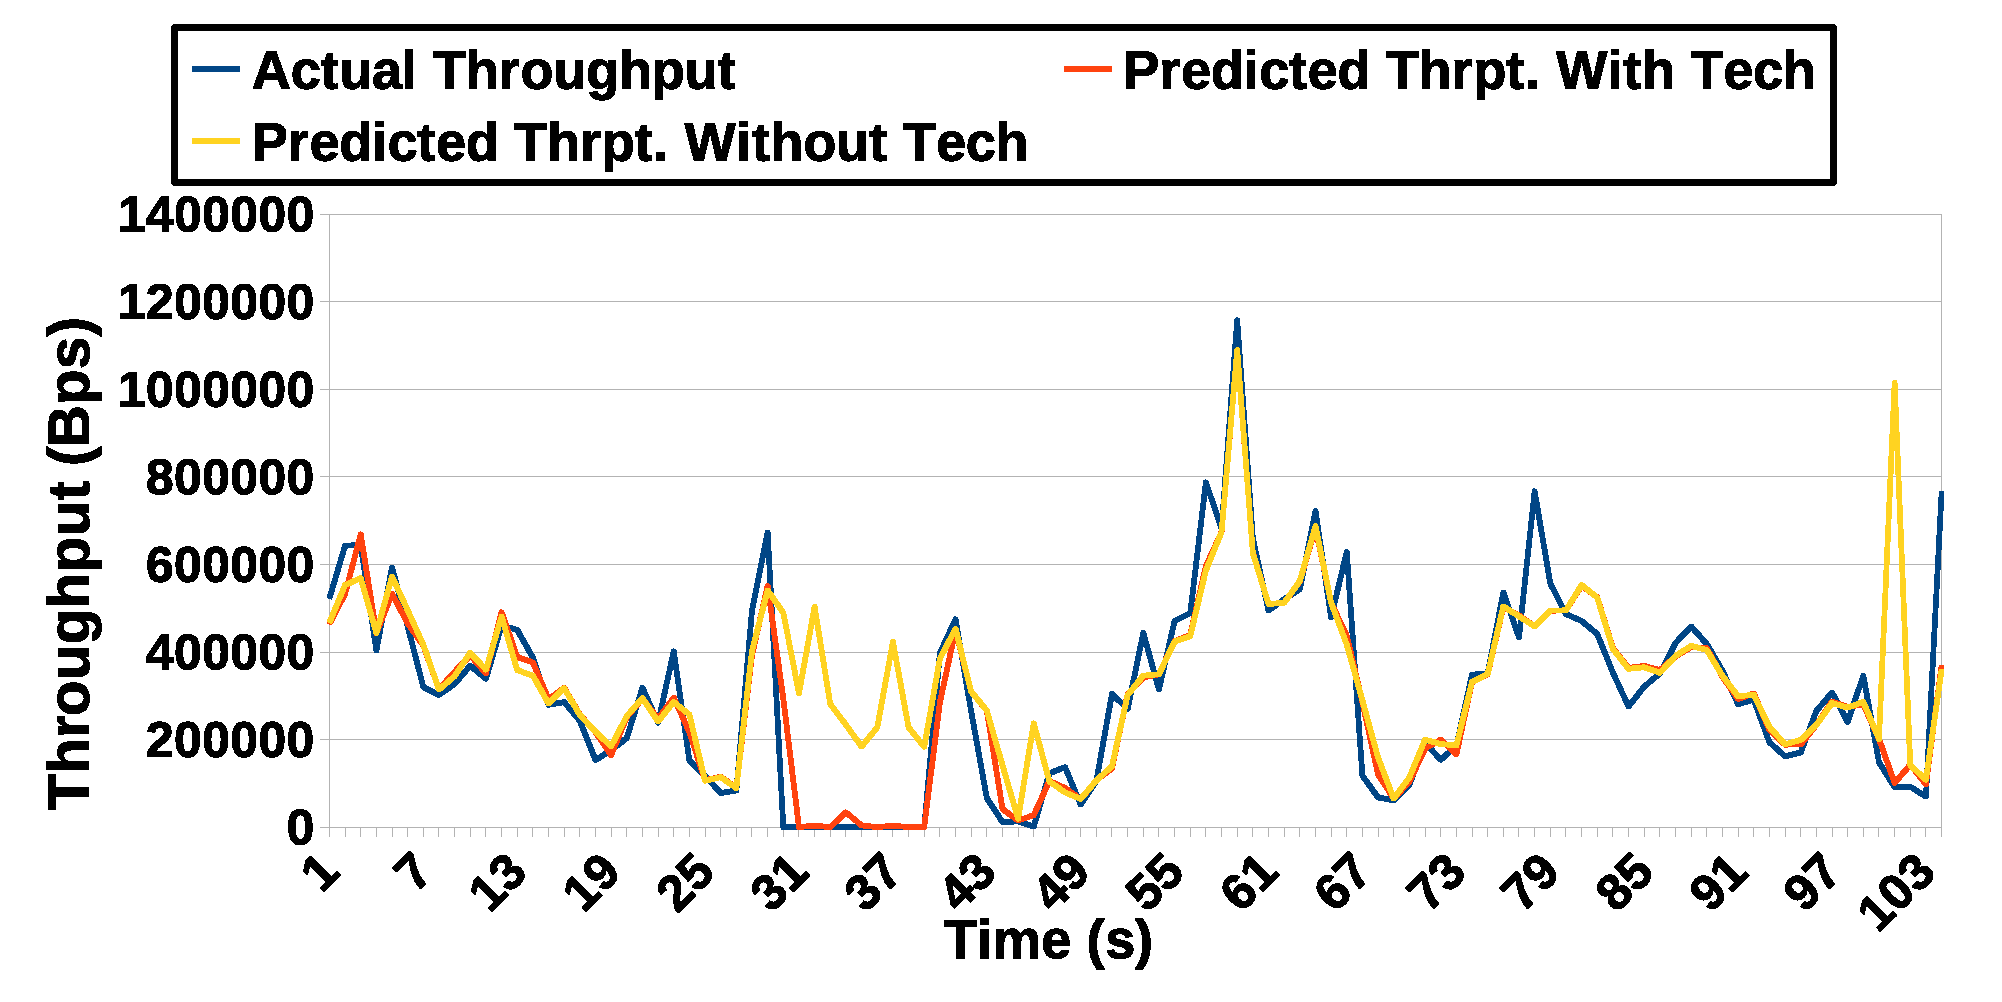
\includegraphics[width=0.3\textwidth]{figures/predicted_vs_actual_vs_Tech.eps}}%
% %\hspace{0.1cm}
% \subfigure[Impact of associated technology on prediction accuracy]{%
% \label{fig:accuracy_pred}%
% 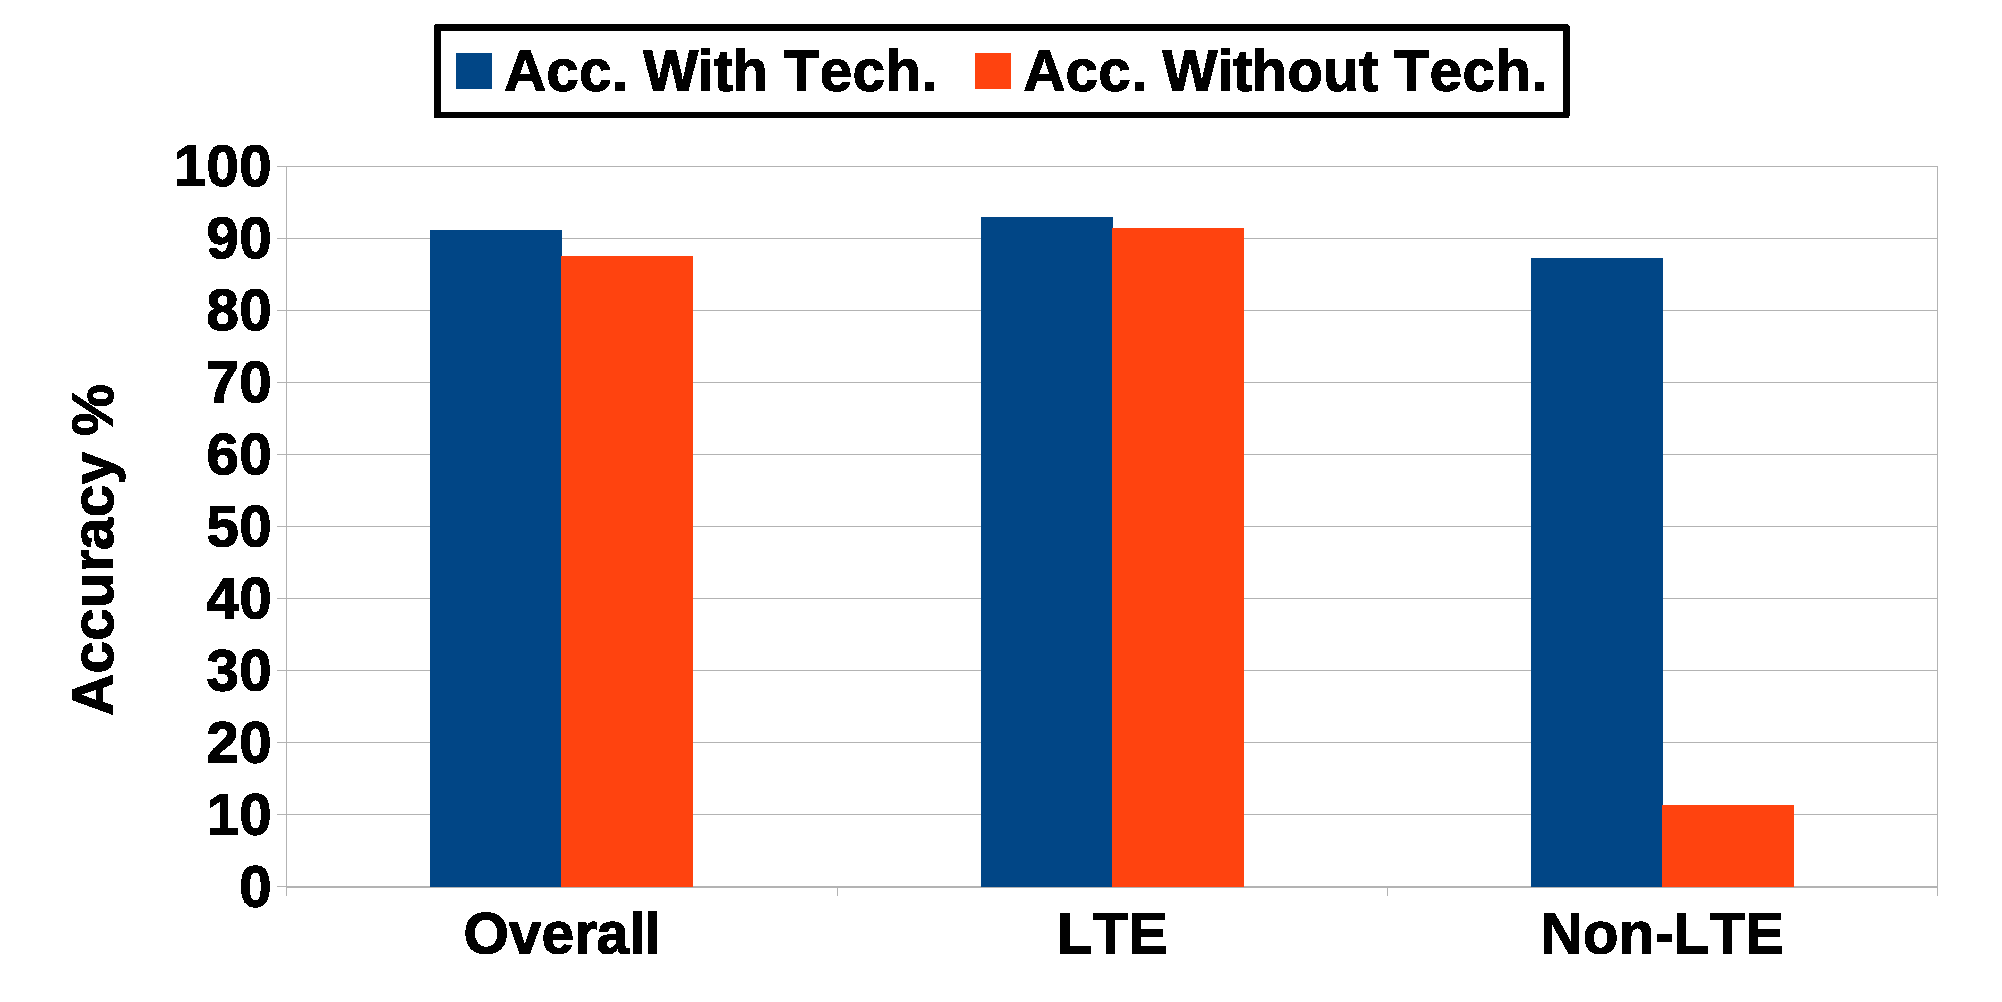
\includegraphics[width=0.3\textwidth]{figures/accuracy_with_vs_without_tech.eps}}%
% \caption{Feature Analysis of the Throughput Prediction Engine}
% \end{figure*}
%  Fig. \ref{fig:feature_imp} shows the weightage of each of the parameters discussed above. We observe that the associated network technology has a significant contribution in the network throughput. This is further confirmed by Fig. \ref{fig:thpt_pred_trace} which shows the actual throughput, and the predicted throughput. It is found that when the associated technologies and the vertical handovers are considered as input parameters, the predicted throughput shows a higher accuracy. Interestingly, Fig. \ref{fig:accuracy_pred} shows that the impact of technology on throughput prediction is the highest for legacy networks. This is primarily because the throughput of the legacy networks is actually very low, and therefore should be accounted for in order to improve \ac{QoE} and energy consumption.

%   \begin{figure}[h]
%      \centering
%      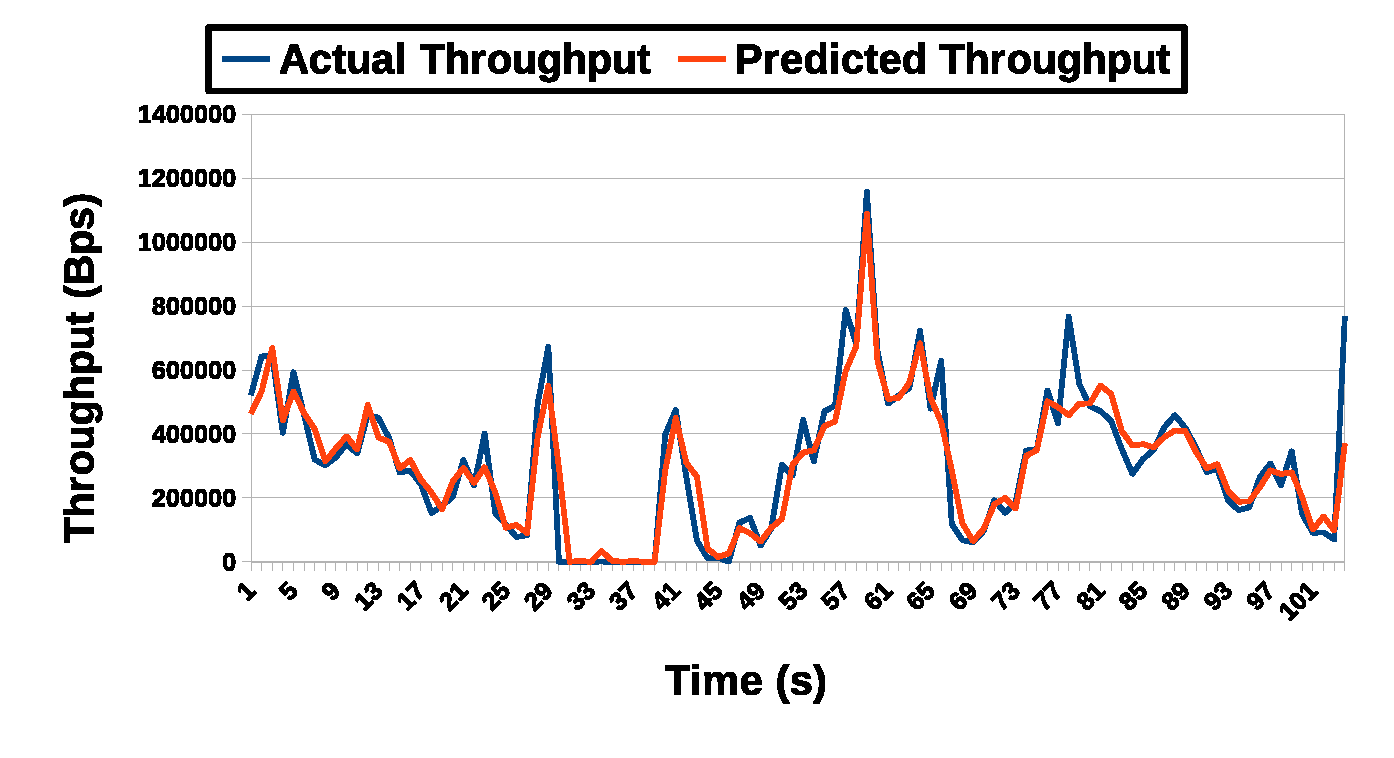
\includegraphics[width=0.5\textwidth]{figures/predicted_vs_actual_thrpt.eps}
%      \caption{The Predicted vs the Actual throughput using the RF algorithm when associated technology is considered. (\basabdatta{\textbf{WE NEED TO SHOW RESULTS OF PREDICTION WITHOUT INCLUDING FEATURE IMPORTANCE AND VERTICAL H/Os}})}
%      \label{fig:thpt_pred_trace1}
%  \end{figure}
 \subsection{The Buffer Length Decision Engine}\label{sec:buff_length_dec_engine}
 %In this section, we describe the design aspects of the buffer and the bitrate decision engines. \\
 \indent The Buffer Length Decision engine also runs at the beginning of each time slot and the playback buffer length is predicted from the predicted network throughput.  However, the relationship between the predicted throughput and the buffer length is not straightforward and is not analytically tractable. So, we employ an A3C \ac{RL} based deep neural network to determine the optimal buffer length.\\ 
 %As mentioned earlier, we run \ac{RL} algorithm to predict the buffer length.  %\basabdatta{The buffer length is tuned to the wireless network throughput. So, it is imperative that the buffer length be tuned accurately to the predicted average throughput, any aberrations from which will initiate a gradual degradation in the opportunities for energy savings and QoE improvement.} {\textcolor{red}{The previous two lines highlighted in blue may be removed.}} However, the relationship between the predicted throughput and the buffer length is not straightforward and hence is not analytically tractable. This encourages us to employ a deep-RL based neural network to reach the buffer length decision.\\
%\indent Since we use an RL algorithm operates on an environment \ti{E}, takes a state \ti{S} as input, responds with an action \ti{A}, and receives reward \ti{R}. 
\indent The components of the \ac{RL} algorithm corresponding to the buffer decision engine are as follows:\\
% \begin{itemize}
\noindent \textbf{(i) Environment}  \ti{E} - video player.\\
\noindent \textbf{(ii) Input state at timeslot \mq{t}} $S_t$ =  ($\hat{\tau}_{{t}}$, $B_{av_t}$, ${\mathcal{X}}$), where
  $\hat{\tau}_{{t}}$ is the  average predicted cellular network throughput,
 $B_{av_t}$ is the current playback buffer capacity available in seconds,
$\mathcal{X}$ is the set of possible changes in buffer length. If the current buffer length is $B_{t-1}$, the next buffer length can be predicted to be $\hat{B_t}= B_t+x$ where $x\in\mathcal{X}:=\{-2,-1,0,+1,+2\}$. $x=1$ implies an increase in buffer length by a single chunk, each chunk is of eight seconds.\\
\noindent \textbf{(iii) Action} $A_t$ - Decisions on the increase or decrease of buffer length at timeslot $t$. \\
\noindent \textbf{(iv) Reward} - The reward function is defined as a linear weighted function of energy savings with respect to a baseline ABR algorithm and the QoE score:
    \begin{equation}
    \Xi_{\mathrm{bufflen}} = w_1 \cdot (\left|E_{\mathrm{EnDASH}_t}-E_{\mathrm{old}_t}\right|)+w_2 \cdot QoE
    \end{equation}
    
% \end{itemize}
\indent The first term in the reward function gives the energy savings with respect to a baseline ABR algorithm. In this work, we have chosen BOLA \cite{Spiteri2016} as the baseline since its energy consumption is the lowest among existing algorithms (excluding EnDASH, \S{\ref{section:evaluation}}).  $E_{\mathrm{old}_t}$ and $E_{\mathrm{EnDASH}_t}$ represent the energy consumption of BOLA and of EnDASH at time \mq{t}, respectively. The energy consumed while using one particular algorithm is obtained as follows:  the RRC states are first identified from the download packet capture of a video trace. Next, the dwell time in each RRC state is multiplied by the corresponding power consumption (obtained from the RRC state machine) to get the energy quantities. We calculate the energy savings in this manner because the ground truth on energy consumption cannot be obtained.\\
%It is obtained as follows. The buffer length decision engine is trained using the power consumption and throughput data traces that we have collected using the Moto G5 phone over the Airtel network. Corresponding to this handset and network combination we have obtained an RRC state machine which gives the power consumptions in the \textit{CONNECTED}, \textit{TAIL}, and \textit{IDLE} RRC states,  as discussed in \S\ref{section:motivation}. From a collected video trace it is possible to identify these state. So, equipped with the RRC state machine it is possible to calculate the energy consumption of any \ac{ABR} streaming algorithm, once the RRC states are identified for any video trace.
\indent Second term in the reward function is the \textbf{\ac{QoE}} metric  \cite{Yin2015}:
\begin{equation}\label{eq:QoE}
   \text{QoE} = \sum_{i=1}^N q(R_i) - \mu\sum_{i=1}^N \delta_i - \sum_{i=1}^{N-1}\left|q(R_{i+1})-q(R_i)\right|
\end{equation}
The $\text{QoE}$ metric is defined for a video with N chunks. $R_i$ is the bitrate of $\text{chunk}_i$ and $q(R_i)$ maps the bitrate to a quantity which represents the quality perceived by the user. We have taken $q(R_i) = R_i$ \cite{mao2017neural}. $\delta_i$ is the rebuffering time involved in downloading $\text{chunk}_i$ at bitrate $R_i$. $\mu$ represents the degree of penalty associated with $\delta_i$.  We have taken $\mu=4.3$ \cite{mao2017neural}. The last term represents the playback smoothness. The QoE decreases when there is abrupt variability in throughput between successive chunks. Thus, QoE increases with bitrate, and reduces with rebuffering time and throughput variability.
\subsection{The Bitrate Decision Engine}
 \label{sec:bitrate_dec_engine}
 %\indent The bitrate decision engine runs every time a video chunk is to be downloaded. \niloy{Isn't this a heavy overhead} 
 %The objective of the bitrate decision engine is to maximize the \ac{QoE} of users. 
 %The output of the buffer decision engine is the length of the playback buffer in terms of the number of video seconds to be played. \niloy{played or stored} This eventually translates into the number of video chunks to be downloaded. So, the higher is the throughput, the higher will be the playback buffer length and hence, the number of chunks that can be downloaded.  It is, therefore, important that the buffer length be tuned accurately to the predicted average throughput, any aberrations from which will initiate a gradual degradation in the opportunities for energy savings and QoE improvement. For enabling an optimal buffer length decision, we, therefore, consider the following parameters as input to the buffer decision engine at the end of time slot \mq{t}:
%   Once the buffer length is tuned to the link throughput, EnDASH progresses towards video chunk downloads.
%  \subsection{The Buffer and Bitrate Decision Engine}
%  \niloy{Buffer has 6 levels. }
%  \subsubsection{Bitrate Decision Engine}\label{sec:bitrate_dec_engine}
%  Decisions on the optimal bitrates for the next video chunk is taken just before downloading the chunk. 
%So, the bitrate decision engine runs asynchronously with respect to the buffer length decision engine, but it needs the available buffer length to make its decision. This makes the EnDASH architecture a cascaded design of the buffer length decision engine followed by the bitrate selection engine. 
The predicted playback buffer length is next used for selecting optimal chunk bitrates using a deep \ac{RL} based algorithm. The components of the \ac{RL} algorithm are:\\
%\begin{itemize}
\noindent\textbf{(i) Environment}  \ti{E} - video player.\\
\noindent\textbf{(ii) Input state before downloading the chunk \mq{n}}, \\$S_{n}$ = ($\hat{\mathcal{B}_t}, \tau_c(n-1)$, $d_{n-1}$, $l_{n-1}$, $B_{n}$, $\zeta_{n}$, $r_{n}$), where $\hat{\mathcal{B}_t}$- predicted playback buffer length for current slot \mq{t}, $\tau_c(n-1)$= throughput of last chunk, $d_{n-1}$ = time taken to download last chunk, $l_{n-1}$ = bitrate of last chunk, $B_{n}$ = available playback buffer length, $\zeta_{n}\in\bracket{s_1,s_2,\cdots s_m}$ = Possible size of next video chunk  ($m$ available sizes), $r_{n+1}\in \bracket{R_1, R_2,\cdots, R_6}$ = Possible bitrate levels for next video chunk.\\
\noindent\textbf{(iii) Action} $A_n$ - Optimal bitrate decision for the next chunk.\\ 
\noindent\textbf{(iv) Reward}- QoE score obtained from eqn. (\ref{eq:QoE}).\\
\indent The buffer length and bitrate decision engines run at two different time scales. So, time slot indices for the variables related to the buffer length decision engine and the bitrate decision engine are denoted by  \mq{t} and \mq{n}, respectively.
 \subsection{Emulation environment for \ac{RL} training}
  In the training phase, the \ac{RL} agent of the buffer and the bitrate decision engine of EnDASH should ideally be trained using real video downloads at actual video streaming clients. 
  %This requires that for a single training data point an entire video chunk should be downloaded. 
  However, this demands that entire chunks be downloaded for each training data point. Further, downloads over cellular networks can be quite slow. Hence, to save training time, we train EnDASH and its competing  ABR algorithms using an emulation environment that closely mimics a real video client application. The emulator maintains its own representation of a real client's playback buffer. At the beginning of a time slot, the emulator first predicts the average throughput and then the playback-buffer length for the slot. Within the slot, once a chunk is to be downloaded, the emulator first assigns a download time to the chunk based  on its bitrate and the internal network throughput, derived from previous chunks. It then depletes the playback-buffer by the chunk's download time to emulate the playback-buffer drainage during an ongoing chunk download. It adds the playback duration of the  chunk being currently downloaded to the playback-buffer. The emulator sleeps temporarily once the playback buffer is full. Rebuffering occurs if the playback-buffer is completely drained before the next chunk download. The emulator keeps track of the rebuffering event and rebuffering time. After each slot (chunk download), the emulator prepares the state $S_t$ ($S_n$) for the \ac{RL} module of the buffer decision (bitrate decision) engines.
 \subsection{The \ac{RL} Training algorithm}
 Both the buffer length and bitrate decision engines of EnDASH are trained using  state-of-the-art actor-critic method, which involves training two neural networks \cite{mao2017neural}: an actor network and a critic network. A3C is a policy gradient \ac{RL} algorithm which estimates the gradient of the total reward from the trajectories of the execution followed by a policy. The action is chosen based on the policy by the actor network while the critic network estimates the advantage of selecting the action by returning a value function. Both networks update their weights in each time step. \\
 \indent Each parameter of the state \ti{S} of both buffer length and bitrate decision engines are passed on to their respective actor and critic network to enable learning of optimal buffer lengths and bitrates by the corresponding \ac{RL} modules~\cite{mao2017neural}.
%\\
%\indent At the end of each time slot, the  \ac{RL} agent of the buffer length decision engine takes the State Input $S_t$ as discussed in  \S\ref{sec:buff_length_dec_engine}. While once a video chunk is downloaded, the \ac{RL} agent  of the bitrate decision engine takes the State $S_n$ as input. $S_n$ is defined in \S\ref{sec:bitrate_dec_engine}. \\
% Once the respective buffer length and bitrate \ac{\ac{RL}} agents receive the states $S_t$ and $S_n$, they take the actions $A_t$ and $A_n$ corresponding to these states. . 
 %The actions are taken by the two engines based on  policies which are defined as a probability distributions over the actions, i.e., $\pi(S_t,A_t)\longrightarrow [0,1]$ and $\pi(S_n,A_n)\longrightarrow [0,1]$. Both the decision engines learn the policy using some neural networks. After each action is taken, the simulated environment provides the corresponding reward to the learning agent, whose objective is to maximize the reward. \\
 %\textbf{Parallel Training:} 
 As in \cite{mao2017neural}, we initiate multiple learning agents to accelerate the training. By default, there are 16 agents. Each agent is designed to experience a different set of input parameters, e.g., network traces. However, the learning agents continuously report  their individual tuples of (state, action, reward)  to a central model, which aggregates them to generate a single model.
\subsection{Implementation of the \ac{RL} modules}

\begin{figure*}[!h]%
 	\centering
 	\subfigure[Energy Consumption]{%
 		\label{fig:EnDASH_en}%
 		\includegraphics[width=0.49\textwidth]{new_results/simres/Energy}}%
 	\subfigure[QoE score (\ref{eq:QoE})]{%
 		\label{fig:EnDASH_QoE}%
 		\includegraphics[width=0.49\textwidth]{new_results/simres/QoE}}%
 	
 	\subfigure[CDF of buffer length]{%
 		\label{fig:EnDASH_buff}%
 		\includegraphics[width=0.49\textwidth]{new_results/simres/BuffOccu}}
 	%\hspace{0.1cm}
 	\caption{Performance comparison of EnDASH with baseline \ac{ABR} streaming algorithms, BOLA \cite{Spiteri2016}, Pensieve \cite{mao2017neural}, Fast MPC \cite{Yin2015}, Robust MPC \cite{Yin2015}}
 	\label{fig:EnDASH_vs_others}
\end{figure*}

\begin{figure*}[!h]%
 	\centering
 	%\hspace{0.1cm}
 	\subfigure[Avg. Bitrates in Mbps]{%
 		\label{fig:avg_bitrate}%
 		\includegraphics[width=0.49\textwidth]{new_results/simres/AvgBitrate}}%
 	%\hspace{0.1cm}
 	\subfigure[Stall Time per segment (in seconds)]{%
 		\label{fig:stall}%
 		\includegraphics[width=0.49\textwidth]{new_results/simres/Stall}}%
 	
 	\subfigure[Bitrate Variation]{%
 		\label{fig:smooth}%
 		\includegraphics[width=0.49\textwidth]{new_results/simres/BitrateVar}}%
 	\caption{Comparison of different components of \ac{QoE} score (average bitrate, stall time, smoothness) of EnDASH with baseline \ac{ABR} streaming algorithms, BOLA \cite{Spiteri2016}, Pensieve \cite{mao2017neural}, Fast MPC \cite{Yin2015}, Robust MPC \cite{Yin2015}}\vspace*{-0.5cm}
 	\label{fig:indi_QoE}
\end{figure*}

The \textit{bitrate selection engine} of EnDASH is adopted from the state-of-the-art Pensieve algorithm \cite{mao2017neural}, which also uses A3C to learn optimal bitrates. We have used a pretrained model provided by Pensieve, albeit with different input states.  The \textit{buffer length decision engine} has been implemented in Tensorflow \cite{Abadi2016}. The engine passes five previous values of the buffer length to a 1D convolution layer (CNN) with 128 filters, each of size 4 with stride 1. The remaining inputs, i.e., predicted link throughput and current available buffer length are passed onto another 1D-CNN having the same shape. Results obtained from these layers are subsequently combined in a hidden layer having 128 neurons and uses the softmax function. The same inputs are also used by the critic network, which has the same neural network, but whose final output is a linear neuron. During the training of the algorithm, we set the discount factor to 0.9, i.e., current actions are allowed to be influenced by 100 future steps. The learning rates for the actor and the critic networks are 0.0001 and 0.001, respectively. The entropy factor $\beta$ has been set to gradually decrease from 1 to 0.1 over iterations.

%\indent In the next section we discuss how the proposed EnDASH system performs in terms of energy savings and QoE with respect to other state-od-the-art \ac{ABR} algorithms.